

\documentclass[11pt]{article}

\usepackage{graphicx} \usepackage{float} \usepackage{epstopdf}
\usepackage{xcolor}

\renewcommand{\baselinestretch}{1.2} \setlength{\topmargin}{-0.5in}
\setlength{\textwidth}{6.5in} \setlength{\oddsidemargin}{0.0in}
\setlength{\textheight}{9.1in}

\newlength{\pagewidth} \setlength{\pagewidth}{6.5in} \pagestyle{empty}

\def\pp{\par\noindent}

\begin{document}

\centerline{\bf CSE 350 -- Theory of Computation (Honors), Spring 2018}
\medskip
\centerline{Assignment 1}
\bigskip
\bigskip

\newcounter{problemctr}

\centerline{\bf Part B}
\addtocounter{problemctr}{1}
\addtocounter{problemctr}{1}
\addtocounter{problemctr}{1}

\addtocounter{problemctr}{1}
\bigskip

\noindent
$\underline{\rm Problem\ \theproblemctr}$\pp Are the following statements true
or false? Justify your answers with a proof or counterexample.

\noindent
(1) If $L_1$ and $L_2$ are both infinite languages, $L_1L_2$ contains a string
that is in neither $L_1$ nor $L_2$.\\

False - in the case where $L1$ and $L2$ are the same language. Another example would be $L_1$ is the language containing all strings with an even number of $a$'s, and $L_2$ is a language containing all strings with an odd number of $a$'s.\\

\noindent
(2) If $L$ is finite, then $|L^*| > |L|$.\\

False - in the case where $L=\{e\}$, $L^*=\{e\}$, $|L^*|=|L|$.

\addtocounter{problemctr}{1}
\bigskip
\noindent
$\underline{\rm Problem\ \theproblemctr}$\pp Prove or disprove: the union of
countably many countably infinite sets is countable.\\

%Aside: You may assume the Axiom of Choice (if you don't know what that means, don't worry).

There exists a method of traversal through the union of countably many countably infinite sets that allows the eventual indexing of any arbitrary element in any of the sets to a natural number.\\
Given an list of sets, as demonstrated below:\\

\begin{tabular}{llllllllll}
$S_1:$ \{& 0,& 0, & 0, & 0, & 0, &. &. &. &\}\\
$S_2:$ \{& 0,& 1,& 2,& 3,& 4,&. &. &. &\}\\
$S_3:$ \{& 0,& 1,& 2,& 1,& 3,&. &. &. &\}\\
$S_4:$ \{& 1,& 1,& 0,& 2,& 1,&. &. &. &\}\\
$S_5:$ \{& 2,& 3,& 4,& 5,& 2,&. &. &. &\}\\
. &. &. &. &. &. &. &. &. &\\
. &. &. &. &. &. &. &. &. &\\
\end{tabular}\\

We traverse the sets in a boustrophedonic pattern as follows, indexing each element in the order in which we encounter them:\\
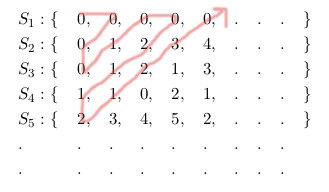
\includegraphics{boust.png}\\
In this method, we can reach any given element in a finite number of steps. We prove that any element can be indexed contained in any of the sets can by a natural number.

\addtocounter{problemctr}{1}
\bigskip
\noindent
$\underline{\rm Problem\ \theproblemctr}$ (Extra Credit)\pp
\noindent
There are $N$ soldiers lined up, about to execute a hapless
prisoner. The lieutenant, who begins the firing process, is
located at one end of the line. The soldiers all want to fire
simultaneously. Unfortunately, the soldiers can only talk to their
immediate neighbors on the left and right. In addition, these
soldiers are not very intelligent, and they are just finite automata.
Thus, they only have {\em constant
memory\/}, independent of $N$. Notice that constant memory is very
little. It is not enough even to count up to $N$; this requires
$\log (n)$ bits. It is not enough to have a name, because unique
names also require $\log (n)$ bits.

\noindent
Devise a procedure that allows these soldiers to fire in unison. The
algorithm should have running time $O(n)$.

\noindent
Note that they move and interact at exactly
the same speed; i.e., they are synchronized.\\

---NOTE---\\

Below is the solution from the practice problems I submitted on Thursday. On further reflection, I realize that multiple "searches" can be simultaneously performed, so rather than it being O(nlogn) as I originally stated, I believe it may be O(n).\\

----------\\

O(nlogn) solution:

First, we establish a method that in O(n) time and requires 2 bits of memory per soldier, finds the middle soldier(s) in the line.\\

The first soldier passes a message that we'll call 'a' down the line. Every soldier who receives it passes it on to the next soldier on the following "turn." When the last soldier receives it, they send it back up the line.

Two turns after the first soldier passes the initial message 'a', they then pass another message 'b' down the line. Every soldier who receives it must wait two turns before passing it on.

The result is that for every three steps 'a' travels down the line, 'b' travels one step. 'b' travels three times slower than 'a', so in the time it takes 'b' to make it halfway down the line, 'a' will have travelled one-and-a-half times the length of the line and be at the halfway point moving back up the line.

If the line has an odd number of soldiers, then the middle soldier will simultaneously receive 'a' and 'b' coming from opposite directions. If the line has an even number of soldiers, then the two middle soldiers may not necessarily receive 'a' and 'b' on the same turn, but if they try and "pass" it along to the next soldier and the soldier is already carrying the other message, then that means the two of them are the middle soldiers.

The time it takes to find the middle soldier(s) is at $\frac{3}{2}n$ or $O(n)$.

Odd-N example below:\\

\begin{tabular}{|l|l|l|l|l|}
    \hline
        a$\rightarrow$&&&&\\
    \hline
        &a$\rightarrow$&&&\\
    \hline
        b$\rightarrow$&&a$\rightarrow$&&\\
    \hline
        &&&a$\rightarrow$&\\
    \hline
        &&&&$\leftarrow$a\\
    \hline
        &b$\rightarrow$&&$\leftarrow$a&\\
    \hline
        &&ab&&\\
    \hline
\end{tabular}

Even-N example below:\\

\begin{tabular}{|l|l|l|l|l|l|}
    \hline
        a$\rightarrow$&&&&&\\
    \hline
        &a$\rightarrow$&&&&\\
    \hline
        b$\rightarrow$&&a$\rightarrow$&&&\\
    \hline
        &b&&a$\rightarrow$&&\\
    \hline
        &b&&&a$\rightarrow$&\\
    \hline
        &b$\rightarrow$&&&&$\leftarrow$a\\
    \hline
        &&b&&$\leftarrow$a&\\
    \hline
        &&b$$&$\leftarrow$a&&\\
    \hline
        &&b&a&&\\
    \hline
\end{tabular}\\

Now that we can find the middle soldier(s) in $O(n)$ time, we can use this to coordinate the firing.

First, imagine each soldier has a bit that is all initially set to 0. In a method similar to mergesort's or quicksort's halfway partitioning method, we first find the middle soldier(s) of the line and have them set their bit(s) to 1, thus dividing the line into two equal parts on either side of the middle soldier(s).

The soldier(s) in the middle then initiate the same $O(n)$ median-search procedure on each side to find the middle soldier(s) of each half and have them set their bits to 1. Repeat this recursively until all the soldiers have their bits set to 1.

Once a soldier and their 2 neighbors (or 1 neighbor in the case of the ones at the ends) have their bits set to 1, then they fire the following turn. The reason this works is because the procedure always flips the bit of the soldier at the halfway point, guaranteeing that the soldiers end up alternating bits before they all flip to 1.

Example below:\\

\begin{tabular}{|l|l|l|l|l|l|l|l|l|l|l|l|l|l|l|l|l|}
    \hline
        1st Search&0&0&0&0&0&0&0&1&0&0&0&0&0&0&0\\
    \hline
        2nd Search&0&0&0&1&0&0&0&1&0&0&0&1&0&0&0\\
    \hline
        3rd Search&0&1&0&1&0&1&0&1&0&1&0&1&0&1&0\\
    \hline
        4th Search&0&1&0&1&0&1&0&1&0&1&0&1&0&1&0\\
    \hline
        5st Search&1&1&1&1&1&1&1&1&1&1&1&1&1&1&1\\
    \hline
        Surrounding Bits Set - Fire&1&1&1&1&1&1&1&1&1&1&1&1&1&1&1\\
    \hline
\end{tabular}\\

The rate at which soldiers are "flipped" doubles every iteration of the search since the middle soldiers each start two new searches. This is a divide-and-conquer strategy that requires $O(log_2n)$ searches to complete.

Since each search is $O(n)$ and there are $O(log_2n)$ searches, the total time complexity of this procedure is $O(nlogn)$.
\end{document}
